\documentclass{extbook}[14pt]
\usepackage{multicol, enumerate, enumitem, hyperref, color, soul, setspace, parskip, fancyhdr, amssymb, amsthm, amsmath, bbm, latexsym, units, mathtools}
\everymath{\displaystyle}
\usepackage[headsep=0.5cm,headheight=0cm, left=1 in,right= 1 in,top= 1 in,bottom= 1 in]{geometry}
\usepackage{dashrule}  % Package to use the command below to create lines between items
\newcommand{\litem}[1]{\item #1

\rule{\textwidth}{0.4pt}}
\pagestyle{fancy}
\lhead{}
\chead{Answer Key for Makeup Progress Quiz -1 Version A}
\rhead{}
\lfoot{7547-2949}
\cfoot{}
\rfoot{Fall 2020}
\begin{document}
\textbf{This key should allow you to understand why you choose the option you did (beyond just getting a question right or wrong). \href{https://xronos.clas.ufl.edu/mac1105spring2020/courseDescriptionAndMisc/Exams/LearningFromResults}{More instructions on how to use this key can be found here}.}

\textbf{If you have a suggestion to make the keys better, \href{https://forms.gle/CZkbZmPbC9XALEE88}{please fill out the short survey here}.}

\textit{Note: This key is auto-generated and may contain issues and/or errors. The keys are reviewed after each exam to ensure grading is done accurately. If there are issues (like duplicate options), they are noted in the offline gradebook. The keys are a work-in-progress to give students as many resources to improve as possible.}

\rule{\textwidth}{0.4pt}

\begin{enumerate}\litem{
Solve the modeling problem below, if possible.

\begin{center}
    \textit{ A new virus is spreading throughout the world. There were initially 8 many cases reported, but the number of confirmed cases has doubled every 2 days. How long will it be until there are at least 10000 confirmed cases? }
\end{center}


The solution is \( \text{About } 21 \text{ days} \), which is option B.\begin{enumerate}[label=\Alph*.]
\item \( \text{About } 15 \text{ days} \)

You modeled the situation with $e$ as the base, but solved correctly otherwise.
\item \( \text{About } 21 \text{ days} \)

* This is the correct option.
\item \( \text{About } 6 \text{ days} \)

You modeled the situation with $e$ as the base and did not apply the properties of log correctly.
\item \( \text{About } 7 \text{ days} \)

You modeled the situation correctly but did not apply the properties of log correctly.
\item \( \text{There is not enough information to solve the problem.} \)

If you chose this option, please contact the coordinator to discuss why you think this is the case.
\end{enumerate}

\textbf{General Comment:} Set up the model the same as in Module 11M. Then, plug in 10000 and solve for $d$ in your model.
}
\litem{
Determine the appropriate model for the graph of points below.

\begin{center}
    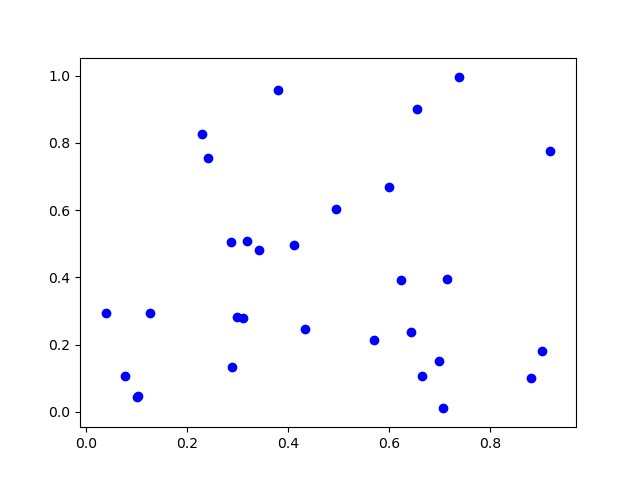
\includegraphics[width=0.5\textwidth]{../Figures/identifyModelGraph12CopyA.png}
\end{center}




The solution is \( \text{None of the above} \), which is option E.\begin{enumerate}[label=\Alph*.]
\item \( \text{Exponential model} \)

For this to be the correct option, we want an extremely slow change early, then a rapid change later.
\item \( \text{Logarithmic model} \)

For this to be the correct option, we want a rapid change early, then an extremely slow change later.
\item \( \text{Non-linear Power model} \)

For this to be the correct option, we need to see a polynomial or rational shape.
\item \( \text{Linear model} \)

For this to be the correct option, we need to see a mostly straight line of points.
\item \( \text{None of the above} \)

For this to be the correct option, we want to see no pattern in the points.
\end{enumerate}

\textbf{General Comment:} This question is testing if you can associate the models with their graphical representation. If you are having trouble, go back to the corresponding Core module to learn about the specific function you are having trouble recognizing.
}
\litem{
For the scenario below, use the model for the volume of a cylinder as $V = \pi r^2 h$ to find the coefficient for the model of the new volume $V_{	ext{new}} = k r^2 h$.

\begin{center}
    \textit{ Pepsi wants to increase the volume of soda in their cans. They've decided to increase the radius by 13 percent and increase the height by 19 percent. They want to model the new volume based on the radius and height of the original cans. }
\end{center}


The solution is \( k = 4.77368 \), which is option B.\begin{enumerate}[label=\Alph*.]
\item \( k = 0.00321 \)

This corresponds to the model: $V = (0.13 r)^2 (0.19 h)$.
\item \( k = 4.77368 \)

* This is the correct option and corresponds to the model: $V = \pi (1.13 r)^2 (1.19 h)$.
\item \( k = 0.01009 \)

This corresponds to the model: $V = \pi (0.13 r)^2 (0.19 h)$.
\item \( k = 1.51951 \)

This corresponds to the model: $V = (1.13 r)^2 (1.19 h)$.
\item \( \text{None of the above.} \)

If you chose this, please talk with the coordinator to discuss why you believe none of the options are correct.
\end{enumerate}

\textbf{General Comment:} When calculating the new dimensions, you need to add/subtract from 100\%. For example, a 10\% increase in height would result in 110\% of the original height: $1.1h_{old} = h_{new}$.
}
\litem{
Determine the appropriate model for the graph of points below.

\begin{center}
    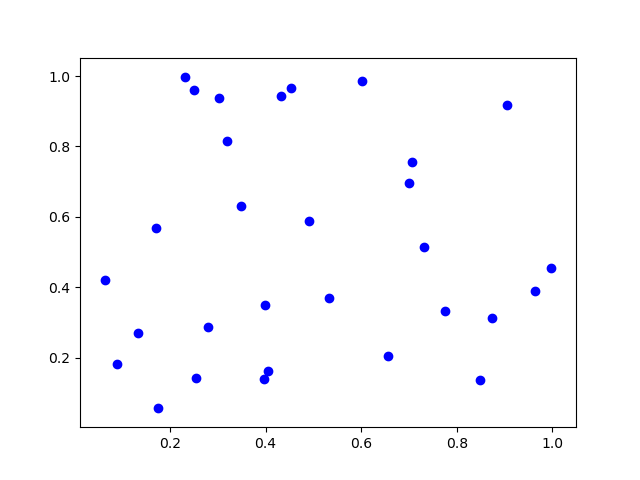
\includegraphics[width=0.5\textwidth]{../Figures/identifyModelGraph12A.png}
\end{center}




The solution is \( \text{None of the above} \), which is option E.\begin{enumerate}[label=\Alph*.]
\item \( \text{Linear model} \)

For this to be the correct option, we need to see a mostly straight line of points.
\item \( \text{Exponential model} \)

For this to be the correct option, we want an extremely slow change early, then a rapid change later.
\item \( \text{Non-linear Power model} \)

For this to be the correct option, we need to see a polynomial or rational shape.
\item \( \text{Logarithmic model} \)

For this to be the correct option, we want a rapid change early, then an extremely slow change later.
\item \( \text{None of the above} \)

For this to be the correct option, we want to see no pattern in the points.
\end{enumerate}

\textbf{General Comment:} This question is testing if you can associate the models with their graphical representation. If you are having trouble, go back to the corresponding Core module to learn about the specific function you are having trouble recognizing.
}
\litem{
Solve the modeling problem below, if possible.

\begin{center}
    \textit{ In CHM2045L, Brittany created a 20 liter 24 percent solution of chemical $\chi$ using two different solution percentages of chemical $\chi$. When she went to write her lab report, she realized she forgot to write the amount of each solution she used! If she remembers she used 12 percent and 27 percent solutions, what was the amount she used of the 12 percent solution? }
\end{center}


The solution is \( 4.00 \), which is option C.\begin{enumerate}[label=\Alph*.]
\item \( 10.00 \)

This would be correct if Brittany used equal parts of each solution.
\item \( 9.13 \)

This was a random value. If this was not a guess, contact the coordinator to talk about how you got this value.
\item \( 4.00 \)

*This is the correct option.
\item \( 16.00 \)

This is the concentration of 27 percent solution.
\item \( \text{There is not enough information to solve the problem.} \)

You may have chose this if you thought you needed to know how much of the second solution was used in the problem. Remember that the total minus the first solution would give you the second amount used.
\end{enumerate}

\textbf{General Comment:} Build the model exactly as you did in Module 9M. Then, solve for the volume you are looking for.
}
\litem{
For the scenario below, use the model for the volume of a cylinder as $V = \pi r^2 h$.

\begin{center}
    \textit{ Pringles wants to add 38 \text{percent} more chips to their cylinder cans and minimize the design change of their cans. They've decided that the best way to minimize the design change is to increase the radius and height by the same percentage. What should this increase be? }
\end{center}


The solution is \( \text{About } 11 \text{ percent} \), which is option C.\begin{enumerate}[label=\Alph*.]
\item \( \text{About } 19 \text{ percent} \)

This corresponds to treating both radius and height as equal contributors and not solving correctly.
\item \( \text{About } 3 \text{ percent} \)

This corresponds to not solving for the increase properly.
\item \( \text{About } 11 \text{ percent} \)

* This is the correct option.
\item \( \text{About } 17 \text{ percent} \)

This corresponds to solving correctly but treating both radius and height as equal contributors to the volume.
\item \( \text{None of the above} \)

If you chose this, please contact the coordinator to discus how you solved the problem.
\end{enumerate}

\textbf{General Comment:} Remember that when plugging the increases of values in, you need to treat it as that percentage above 100. For example, a 5 percent increase means 105 percent.
}
\litem{
For the information provided below, construct a linear model that describes her total budget, $B$, as a function of the number of months, $x$ she is at UF.

\begin{center}
    \textit{ Aubrey is a college student going into her first year at UF. She will receive Bright Futures, which covers her tuition plus a \$400 educational expense each year. Before college, Aubrey saved up \$5000. She knows she will need to pay \$700 in rent a month, \$80 for food a week, and \$40 in other weekly expenses. }
\end{center}


The solution is \( \text{none of the above.} \), which is option E.\begin{enumerate}[label=\Alph*.]
\item \( B(x) = 5000 x + 400 \)

This treats the savings as something you get every month rather than a 1-time payment and is modeling Income, not Budget.
\item \( B(x) = 5400 - 1180 x \)


\item \( B(x) = 5400 - 820 x \)

This treats weekly expenses as month expenses rather than multiplying each weekly expense.
\item \( B(x) = 400 x + 5000 \)

This treats the educational expense as something you get every month rather than a 1-time payment and is modeling Income, not Budget.
\item \( \text{None of the above.} \)

* This is the correct option as the model should be $B(x) = 1180 - 5400 x$.
\end{enumerate}

\textbf{General Comment:} This is a Costs, Profit, Revenue question! The most common issues here are: (1) not converting the weekly costs to monthly costs, (2) treating the one-time values like savings and educational expense as happening per month, and (3) not checking that your model is for cost, profit [income], or revenue [budget].
}
\litem{
Solve the modeling problem below, if possible.

\begin{center}
    \textit{ A new virus is spreading throughout the world. There were initially 4 many cases reported, but the number of confirmed cases has doubled every 5 days. How long will it be until there are at least 100000 confirmed cases? }
\end{center}


The solution is \( \text{About } 74 \text{ days} \), which is option D.\begin{enumerate}[label=\Alph*.]
\item \( \text{About } 25 \text{ days} \)

You modeled the situation with $e$ as the base and did not apply the properties of log correctly.
\item \( \text{About } 51 \text{ days} \)

You modeled the situation with $e$ as the base, but solved correctly otherwise.
\item \( \text{About } 28 \text{ days} \)

You modeled the situation correctly but did not apply the properties of log correctly.
\item \( \text{About } 74 \text{ days} \)

* This is the correct option.
\item \( \text{There is not enough information to solve the problem.} \)

If you chose this option, please contact the coordinator to discuss why you think this is the case.
\end{enumerate}

\textbf{General Comment:} Set up the model the same as in Module 11M. Then, plug in 100000 and solve for $d$ in your model.
}
\litem{
Solve the modeling problem below, if possible.

\begin{center}
    \textit{ In CHM2045L, Brittany created a 22 liter 7 percent solution of chemical $\chi$ using two different solution percentages of chemical $\chi$. When she went to write her lab report, she realized she forgot to write the amount of each solution she used! If she remembers she used 5 percent and 16 percent solutions, what was the amount she used of the 5 percent solution? }
\end{center}


The solution is \( 18.00 \), which is option C.\begin{enumerate}[label=\Alph*.]
\item \( 4.00 \)

This is the concentration of 16 percent solution.
\item \( 11.00 \)

This would be correct if Brittany used equal parts of each solution.
\item \( 18.00 \)

*This is the correct option.
\item \( 13.63 \)

This was a random value. If this was not a guess, contact the coordinator to talk about how you got this value.
\item \( \text{There is not enough information to solve the problem.} \)

You may have chose this if you thought you needed to know how much of the second solution was used in the problem. Remember that the total minus the first solution would give you the second amount used.
\end{enumerate}

\textbf{General Comment:} Build the model exactly as you did in Module 9M. Then, solve for the volume you are looking for.
}
\litem{
For the scenario below, use the model for the volume of a cylinder as $V = \pi r^2 h$.

\begin{center}
    \textit{ Pringles wants to add 36 \text{percent} more chips to their cylinder cans and minimize the design change of their cans. They've decided that the best way to minimize the design change is to increase the radius and height by the same percentage. What should this increase be? }
\end{center}


The solution is \( \text{About } 11 \text{ percent} \), which is option A.\begin{enumerate}[label=\Alph*.]
\item \( \text{About } 11 \text{ percent} \)

* This is the correct option.
\item \( \text{About } 17 \text{ percent} \)

This corresponds to solving correctly but treating both radius and height as equal contributors to the volume.
\item \( \text{About } 18 \text{ percent} \)

This corresponds to treating both radius and height as equal contributors and not solving correctly.
\item \( \text{About } 3 \text{ percent} \)

This corresponds to not solving for the increase properly.
\item \( \text{None of the above} \)

If you chose this, please contact the coordinator to discus how you solved the problem.
\end{enumerate}

\textbf{General Comment:} Remember that when plugging the increases of values in, you need to treat it as that percentage above 100. For example, a 5 percent increase means 105 percent.
}
\end{enumerate}

\end{document}